\chapter{Capa de neblina o niebla}

Una vez definidos los sensores a utilizar y sus posiciones en la capa anterior, se va a investigar en la capa de neblina o niebla. En esta se va a buscar un controlador que pueda usarse para recopilar toda la información que los sensores envíen, y prepararla para enviar a la siguiente capa.

\section{Selección de controlador}

Se han analizado las diferentes opciones de controladores que hay para estos sensores y que puedan funcionar dentro de las temperaturas especificadas. La mejor opción es usar un controlador Arduino.

Arduino es una plataforma de hardware libre, basada en una placa con un microcontrolador y un entorno de desarrollo, diseñada para facilitar el uso de la electrónica en proyectos multidisciplinares.

Un controlador Arduino es una placa PCB (Superficie constituida por caminos, pistas o buses de material conductor laminadas sobre una base no conductora) con diferentes entradas y salidas digitales y analógicas, además de salida de voltaje y otras que se necesitarán para el correcto funcionamiento de los sensores.

Existen muchos modelos de placas Arduino. Cada uno tiene sus ventajas e inconvenientes. Por ejemplo, la Arduino Mega que es la más potente y la que más pines de entrada y salida tiene, o la Arduito Ethernet, que incorpora un puerto Ethernet y se puede conectar a la red a través de él. 

%Aplicar efecto a las demás páginas


Para este proyecto se han utilizado dos modelos diferentes:

\begin{figure}[h] 
    \centering
    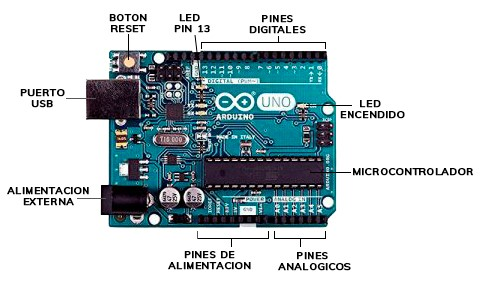
\includegraphics[width=.70\textwidth]{capitulos/capitulo6/uno.jpg}
    \caption{Controlador Arduino Uno.}
    \label{fig:uno}
\end{figure}

\begin{itemize}
    \item \textbf{Arduino UNO:} Es una placa electrónica basada en el microcontrolador ATmega328p. Cuenta con 14 entradas/salidas digitales y otras 6 son entradas analógicas. Además, incluye un resonador cerámico de 16 MHz, un conector USB, un conector de alimentación, una cabecera ICSP y un botón de reseteado. La placa incluye todo lo necesario para que el microcontrolador haga su trabajo, basta con conectarla a un ordenador con un cable USB o a la corriente eléctrica a través de un transformador. En la Figura \ref{fig:uno}, se muestra la placa explicada y las posiciones de los pines.
\end{itemize}

\newpage
\fancyhead{}
\fancyfoot{}
\renewcommand{\headrulewidth}{0.5pt}
\fancyhead[LE,RO]{\textsl{\thepage}}
\fancyhead[RE]{\textsl{\nouppercase{\leftmark}}}
\fancyhead[LO]{\textsl{\nombreTFG}}
Las especificaciones técnicas del controlador se muestran en la Tabla 6.1.

\begin{table}[h]
    \centering
    \begin{tabular}{|l|c|}
        \rowcolor[gray]{.5}
        \hline
        \color{white}Característica & \color{white}Valor \\
        \hline
        Microcontrolador & ATmega328p \\
        \hline
        Voltaje Operativo & 5v \\
        \hline
        Voltaje de Entrada  & de 7 a 12 v \\
        \hline
        Pines de Entradas/Salidas Digital & 14 \\
        \hline
        Pines de Entradas Análogas & 6 \\
        \hline
        Memoria Flash & 32 KB \\
        \hline
        SRAM & 2 KB \\
        \hline
        EEPROM & 1 KB \\
        \hline
        Velocidad del Reloj & 16 MHZ \\
        \hline
    \end{tabular}
    \caption{Especificaciones técnicas del Arudino Uno}
    \label{tab:arduinouno}
\end{table}

La placa Arduino UNO se utilizó al inicio del proyecto para la realización de pruebas. El inconveniente que tuvo era que necesitaba estar conectada por cable, cosa que había que solucionar porque  para la conexión con la siguiente capa tenía que ser sin cable, por lo que se cambió a la segunda placa para realizar una conexión a través de un protocolo inalámbrico.

\begin{figure}[h] 
    \centering
    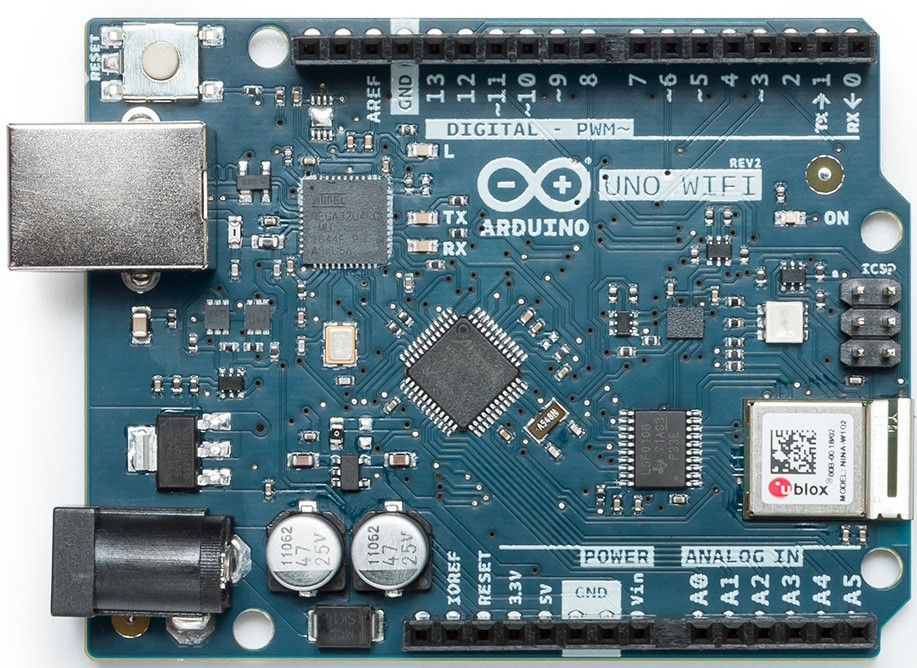
\includegraphics[width=.45\textwidth]{capitulos/capitulo6/unowifi.jpg}
    \caption{Controlador Arduino Uno WiFi rev2.}
    \label{fig:unowifi}
\end{figure}

\begin{itemize}
    \item \textbf{Arduino UNO WiFi rev2:} Como se puede ver, se trata de una Arduino UNO que monta otro chip (ATmega4809). Esta placa incluye mejoras como que cuenta con acelerómetros, un giroscopio y un módulo ESP32 de serie, que permite conexiones como WiFi o Bluetooth. Las conexiones con pines son muy parecidas. En la Figura \ref{fig:unowifi}, se muestra la placa explicada y las posiciones de los pines.
\end{itemize}

Las especificaciones técnicas del controlador se muestran en la Tabla 6.2.

\begin{table}[h]
    \centering
    \begin{tabular}{|l|c|}
        \rowcolor[gray]{.5}
        \hline
        \color{white}Característica & \color{white}Valor \\
        \hline
        Microcontrolador & ATmega4809 \\
        \hline
        Voltaje Operativo & 5v \\
        \hline
        Voltaje de Entrada  & de 7 a 12 v \\
        \hline
        Pines de Entradas/Salidas Digital & 14 \\
        \hline
        Pines de Entradas Análogas & 6 \\
        \hline
        Memoria Flash & 48 KB \\
        \hline
        SRAM & 6 KB \\
        \hline
        EEPROM & 0.25 KB \\
        \hline
        Velocidad del Reloj & 16 MHZ \\
         \hline
    \end{tabular}
    \caption{Especificaciones técnicas del Arudino Uno WiFI rev2}
    \label{tab:arduinounoeifi}
\end{table}

\section{Formas de comunicación}

A continuación, se van a explicar los diferentes protocolos seguidos para la comunicación entre el controlador y el back-end del sistema.

\subsection{Cable}

Este protocolo se usó al principio del proyecto junto con el Arduino UNO para hacer pruebas entre los sensores y afirmar su correcto funcionamiento. 

La comunicación entre el controlador y el back-end del sistema se creaba con un cable conectado al puerto USB de la Arduino Uno, y usando una librería de Arduino llamada \textbf{SerialPort}\cite{twentninth}, la cual enviaba todo lo que se imprimía en el monitor serie, por lo que la información de los sensores se enviaba al back-end imprimiendo en el monitor directamente la información que querías enviar.

Con el avance del proyecto se ha visto necesario que la comunicación entre el controlador y el back-end sea inalámbrica, por lo que se cambió el protocolo de comunicación.

\subsection{WiFi}

Para implementar la comunicación WiFi se necesita un controlador que pueda conectarse a una red de forma inalámbrica, por esto se produce el cambio de un controlador a otro.

La conexión entre el controlador y el back-end ha mejorado. Ahora se utiliza la librería llamada \textbf{WiFiNINA}\cite{thirtieth} para crear una conexión, y la librería llamada \textbf{WiFiUDP}\cite{thirtysecond} para enviar y recibir paquetes UDP del back-end.

Los sensores siguen conectándose a la Arduino de la misma manera, excepto el RFID, que hubo que cambiar las conexiones. Esto se puede ver en el siguiente apartado.

\section{Conexión entre sensores y controladores}

Una vez explicado el controlador a usar y como se va a conectar con el back-end, se va a explicar la conexión entre el controlador y los diferentes sensores.

Para este proyecto se van a utilizar cinco controladores Arduino Uno WiFi rev2, cada una va a tener una IP para identificarse, y un puerto único por el que comunicarse con el back-end.

Los controladores se van a colocar en diferentes puntos del frigorífico para poder recoger la información de los diferentes sensores. En total se van a usar cinco controladores diferentes.

\subsection{Primer controlador}

El primer controlador se va a encargar de gestionar el RFID. Ëste tendrá la IP \textbf{192.168.1.226} y se comunicará con el back-end a través del puerto \textbf{41324}.

La conexión entre pines que había con este sensor y el primer controlador era muy sencilla. Dos de ellos eran para alimentación y los demás a pines digitales.

\begin{figure}[h] 
    \centering
    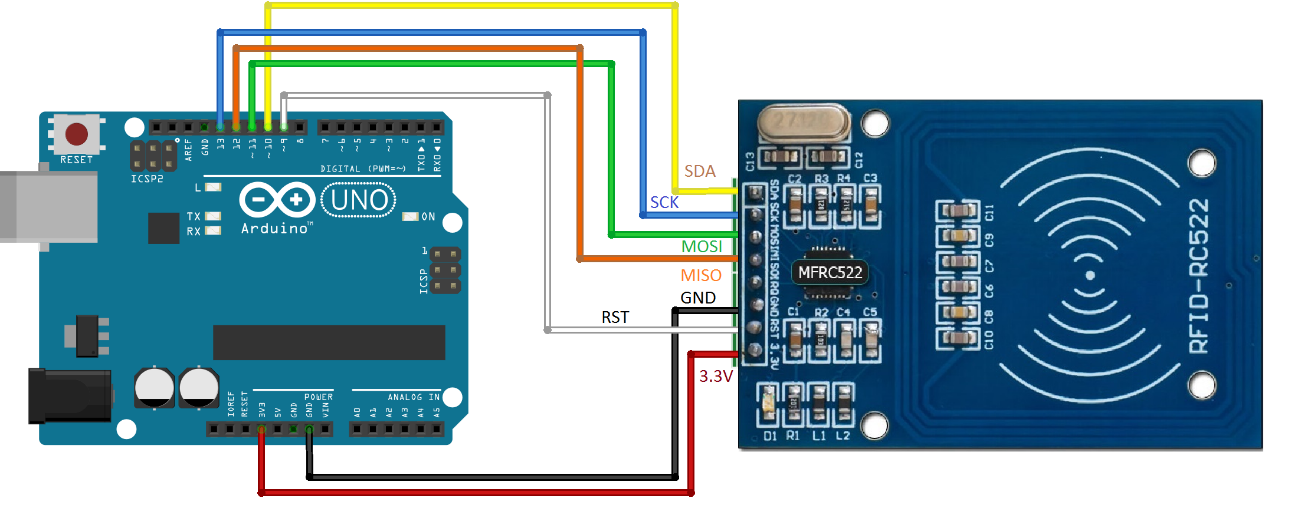
\includegraphics[width=.80\textwidth]{capitulos/capitulo6/ardunorfid.png}
    \caption{Conexión entre Arduino Uno y el sensor RFID.}
    \label{fig:unorfid}
\end{figure}

\newpage
Al cambiar de placa, esto se complicó, porque conectando todo de la misma manera no llegaba a funcionar, por lo que hubo que cambiar la configuración de conexión para su correcto funcionamiento. También se aprovechó y se añadieron algunos LEDs para dar información mientras se hacía uso de este sensor.

En el Arduino Uno WiFi rev2, las conexiones de los pines MISO, MOSI y SCK no son en las mismas posiciones que en la placa anterior. Para conectarla en esta hay que hacer uso del ISCP\cite{thirtyfirst}, que son unos pines del controlador que se puede ver la Figura \ref{fig:iscp}.

Como se ve en la figura mencionada, de aquí se puede obtener los pines que nos faltan para poder conectar el RFID y que funciones correctamente. De esta manera, conectando el sensor RFID de manera correcta, y añadiendo los pines necesarios para añadir los LEDs que se nos darán información, la conexión final se queda como se muestra en la Figura \ref{fig:ard1}.

\begin{figure}[h] 
    \centering
    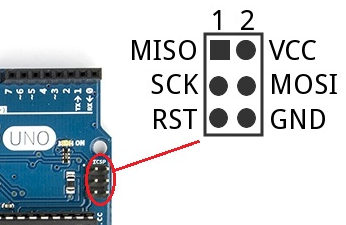
\includegraphics[width=.40\textwidth]{capitulos/capitulo6/iscp.png}
    \caption{ISCP del Arduino Uno WiFi rev2.}
    \label{fig:iscp}
\end{figure}

\begin{figure}[h] 
    \centering
    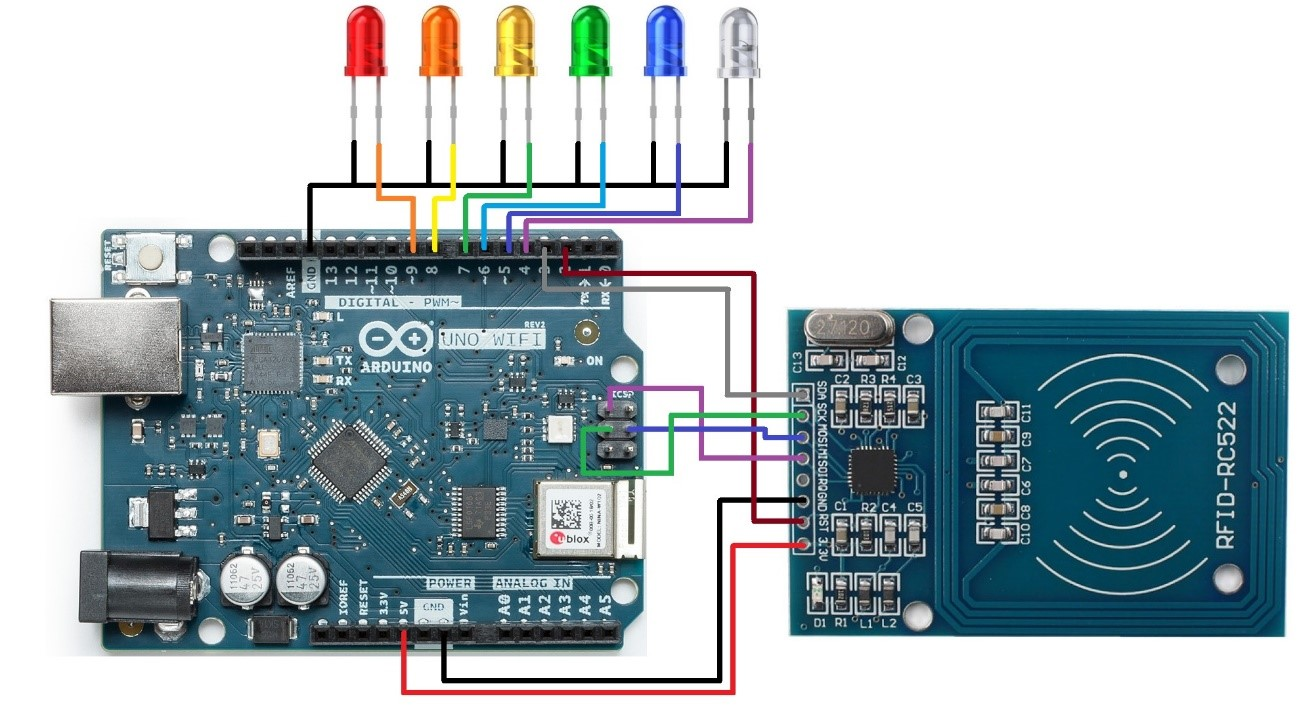
\includegraphics[width=.75\textwidth]{capitulos/capitulo6/ardunowifirfid.jpg}
    \caption{Conexión entre Arduino Uno WiFi rev2 y el sensor RFID.}
    \label{fig:ard1}
\end{figure}

\newpage
Como se puede ver, el RFID está conectado a una toma a tierra (GND) y a una toma de 5V para la alimentación, luego el pin MISO, MOSI y SCK los coge del ISCP, y luego el pin SDA y RST en los puertos digitales 2 y 3.

La conexión de los LEDS a los pines son los siguientes:

\begin{itemize}
    \item El LED blanco que está conectado en el pin digital 4, se ilumina cuando la tarjeta esta siendo usada, por lo que no se puede despegar la tarjeta del lector.
    \item El LED azul que está conectado en el pin digital 5, es cuando un usuario se ha escrito con éxito en una tarjeta y ya puede usarse para identificarse, o cuando un producto ha sido escrito en la tarjeta con éxito y está preparado para meterlo en el frigorífico.
    \item El LED verde que está conectado en el pin digital 6, es cuando un producto ha sido borrado de la tarjeta con éxito y se ha sacado del frigorífico y la tarjeta se queda en blanco para otro uso. 
    \item El LED amarillo que está conectado en el pin digital 7, es cuando un usuario ha sido borrado de la tarjeta con éxito y la tarjeta se queda en blanco para otro uso.
    \item El LED naranja que está conectado en el pin digital 8, es cuando un usuario se ha registrado con éxito en el frigorífico y puede coger cualquier producto que se quedará registra-do con su usuario.
    \item El LED rojo que está conectado en el pin digital 9, es que ha habido un error interno en la lectura/escritura de la tarjeta y hay que intentarlo de nuevo.
\end{itemize}

\subsection{Segundo controlador}

El segundo controlador se va a encargar de gestionar el contenido de los dos cajones de la verdura, es decir, va a gestionar los datos de dos pesos. Éste tendrá la IP \textbf{192.168.1.227} y se comunicará con el back-end a través del puerto \textbf{41325}. La conexión de los pines que hay entre estos dos sensores y el segundo controlador se puede ver en al Figura \ref{fig:ard2}.

\begin{figure}[h] 
    \centering
    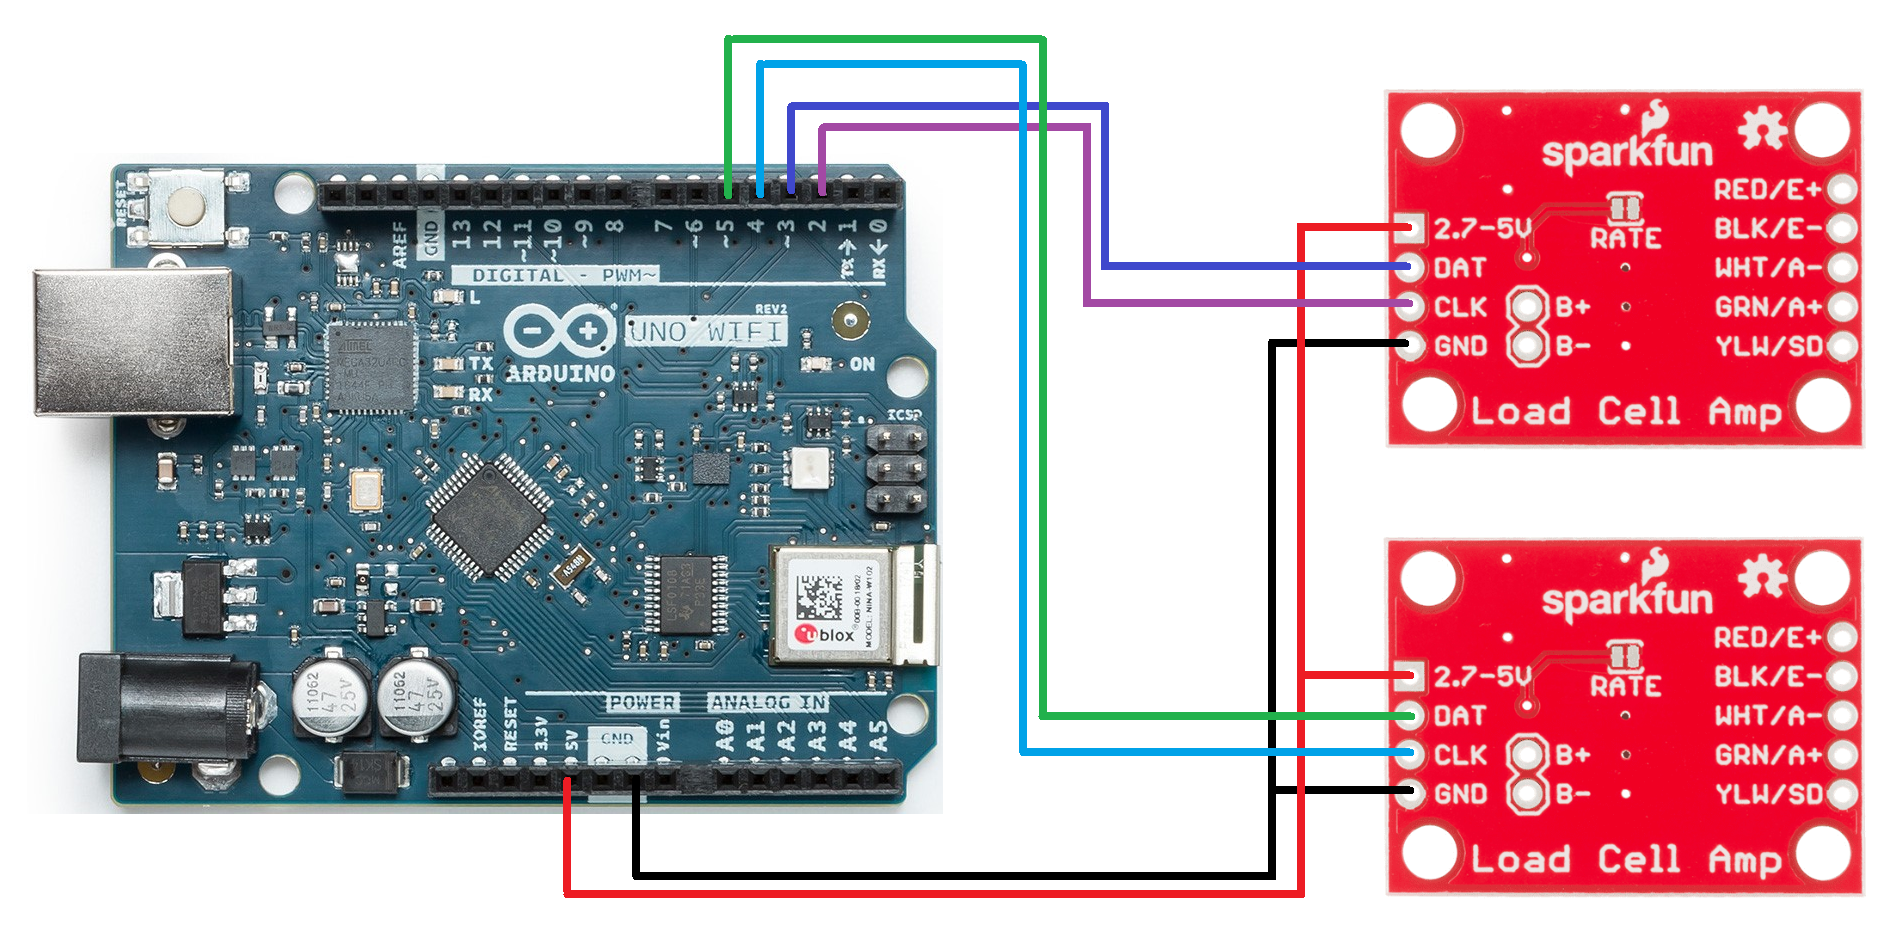
\includegraphics[width=.60\textwidth]{capitulos/capitulo6/ard2.png}
    \caption{Conexión entre Arduino y sensores del cajón de verduras.}
    \label{fig:ard2}
\end{figure}

\newpage
Como se puede ver, cada peso está conectado a una toma a tierra (GND) y a una toma de 5V para la alimentación, luego un peso tiene su pin del reloj al pin digital 2, y el de datos al pin digital 3, el otro peso, el reloj al pin digital 4, y el de datos al pin digital 5.

\subsection{Tercer controlador}

El tercer controlador se va a encargar de gestionar el contenido del cajón del embutido, ósea que va a gestionar dos pesos. Además, también va a gestionar el sensor de nivel de líquidos y los dos receptores de los sensores magnéticos de la puerta. Éste tendrá la IP \textbf{192.168.1.228} y se comunicará con el back-end a través del puerto \textbf{41326}. La conexión de los pines que hay entre estos cinco sensores y el tercer controlador es la mostrada en la Figura \ref{fig:ard3}.

Como se puede apreciar en la Figura \ref{fig:ard3}, cada peso, el sensor de agua y los dos receptores están conectado a una toma a tierra (GND) y a una toma de 5V para la alimentación, luego un peso tiene su pin del reloj al pin digital 2, y el de datos al pin digital 3, el otro peso, el reloj al pin digital 5, y el de datos al pin digital 6. El pin digital 4 está reservado para la entrada de datos del nivel de agua, y el pin 7 y 8 para los receptores.

\begin{figure}[h] 
    \centering
    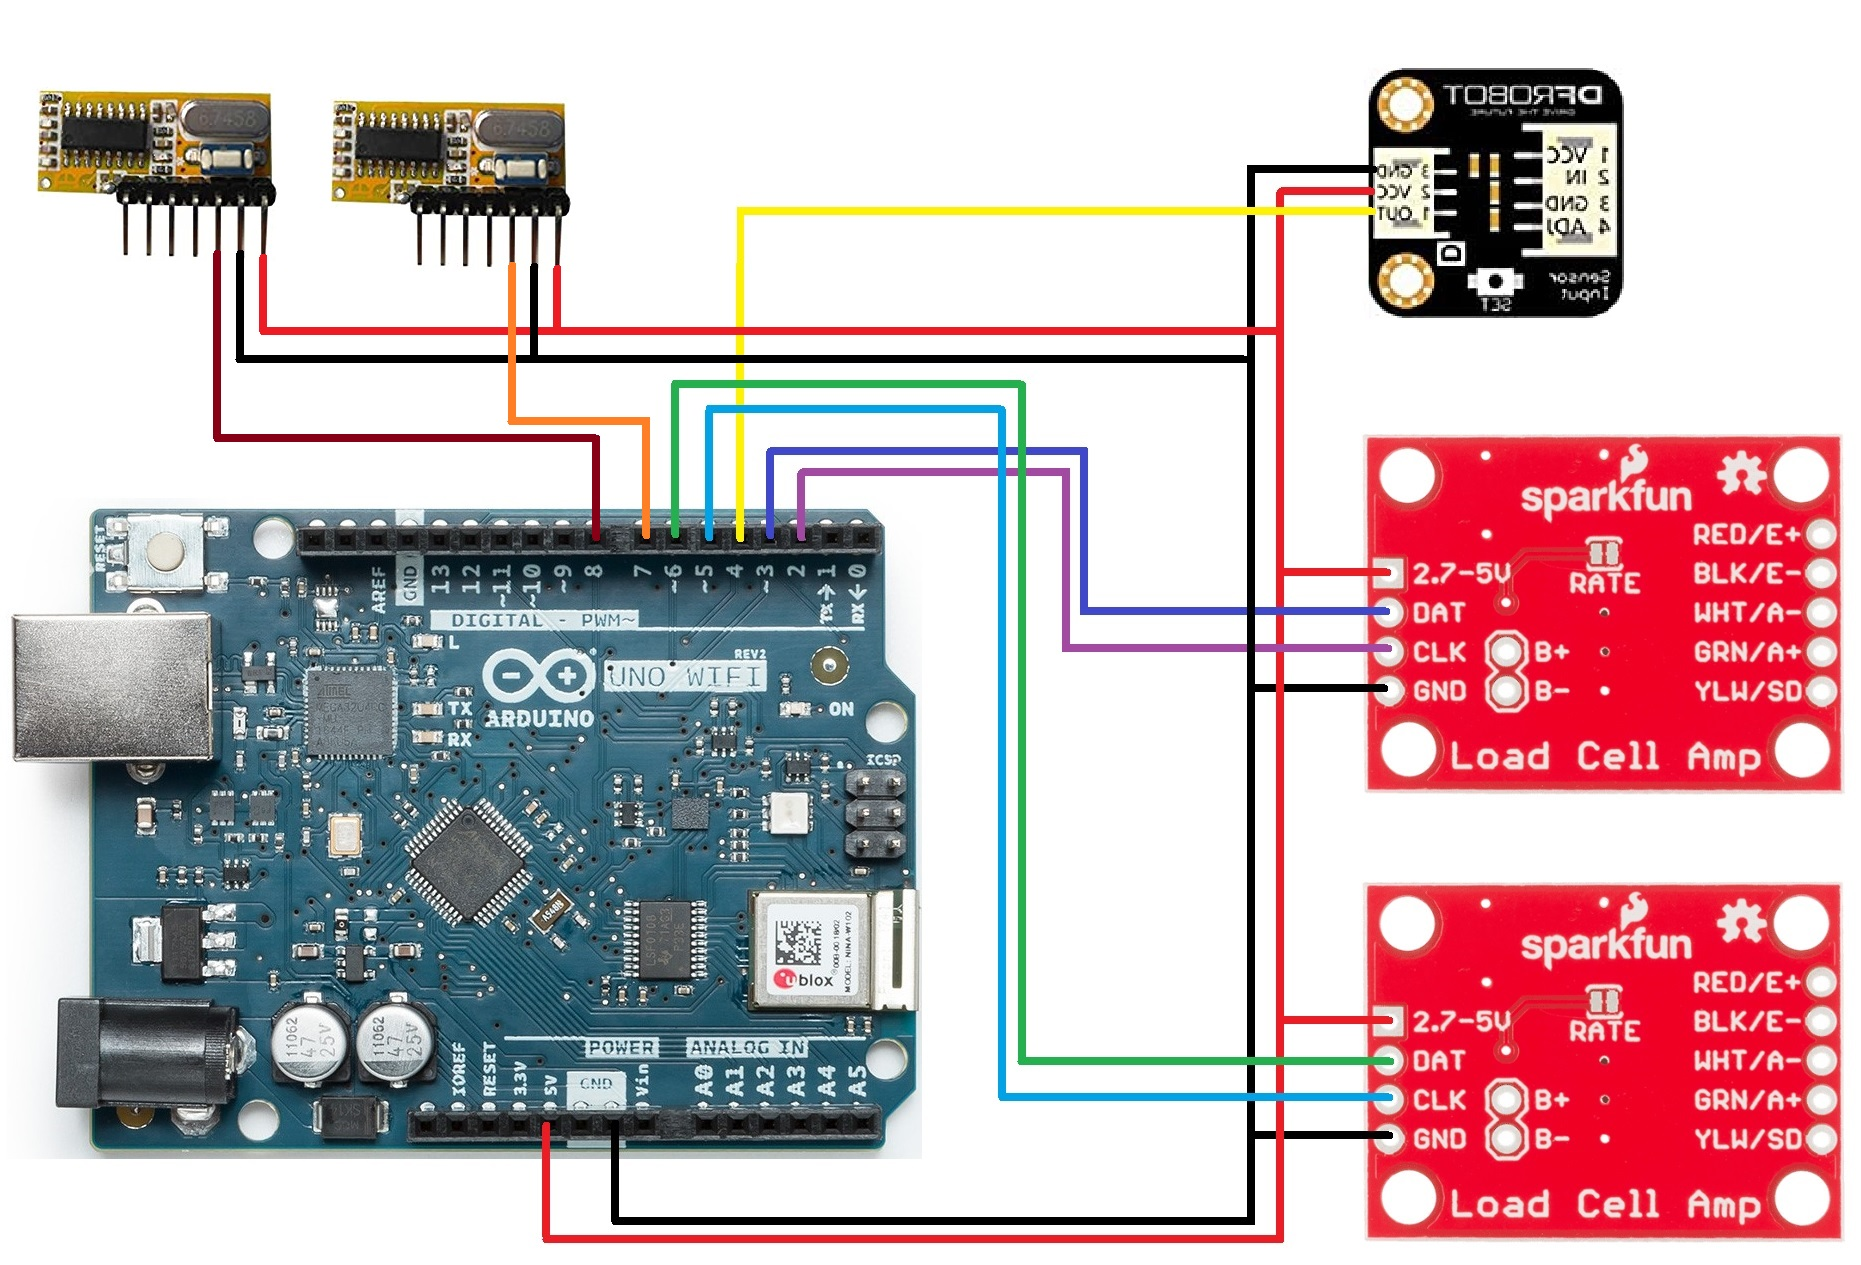
\includegraphics[width=.54\textwidth]{capitulos/capitulo6/ard3.jpg}
    \caption{Conexión entre Arduino y sensores del cajón de embutido y nivel de agua.}
    \label{fig:ard3}
\end{figure}

%\newpage
\subsection{Cuarto controlador}
El cuarto controlador se va a encargar de gestionar el contenido del basar de los huevos, de los refrescos y el de la leche, o sea que va a gestionar seis pesos. Éste tendrá la IP \textbf{192.168.1.229} y se comunicará con el back-end a través del puerto \textbf{41327}. La conexión de los pines que hay entre estos seis sensores y el cuarto controlador es la mostrada en la Figura \ref{fig:ard4}.

\begin{figure}[h] 
    \centering
    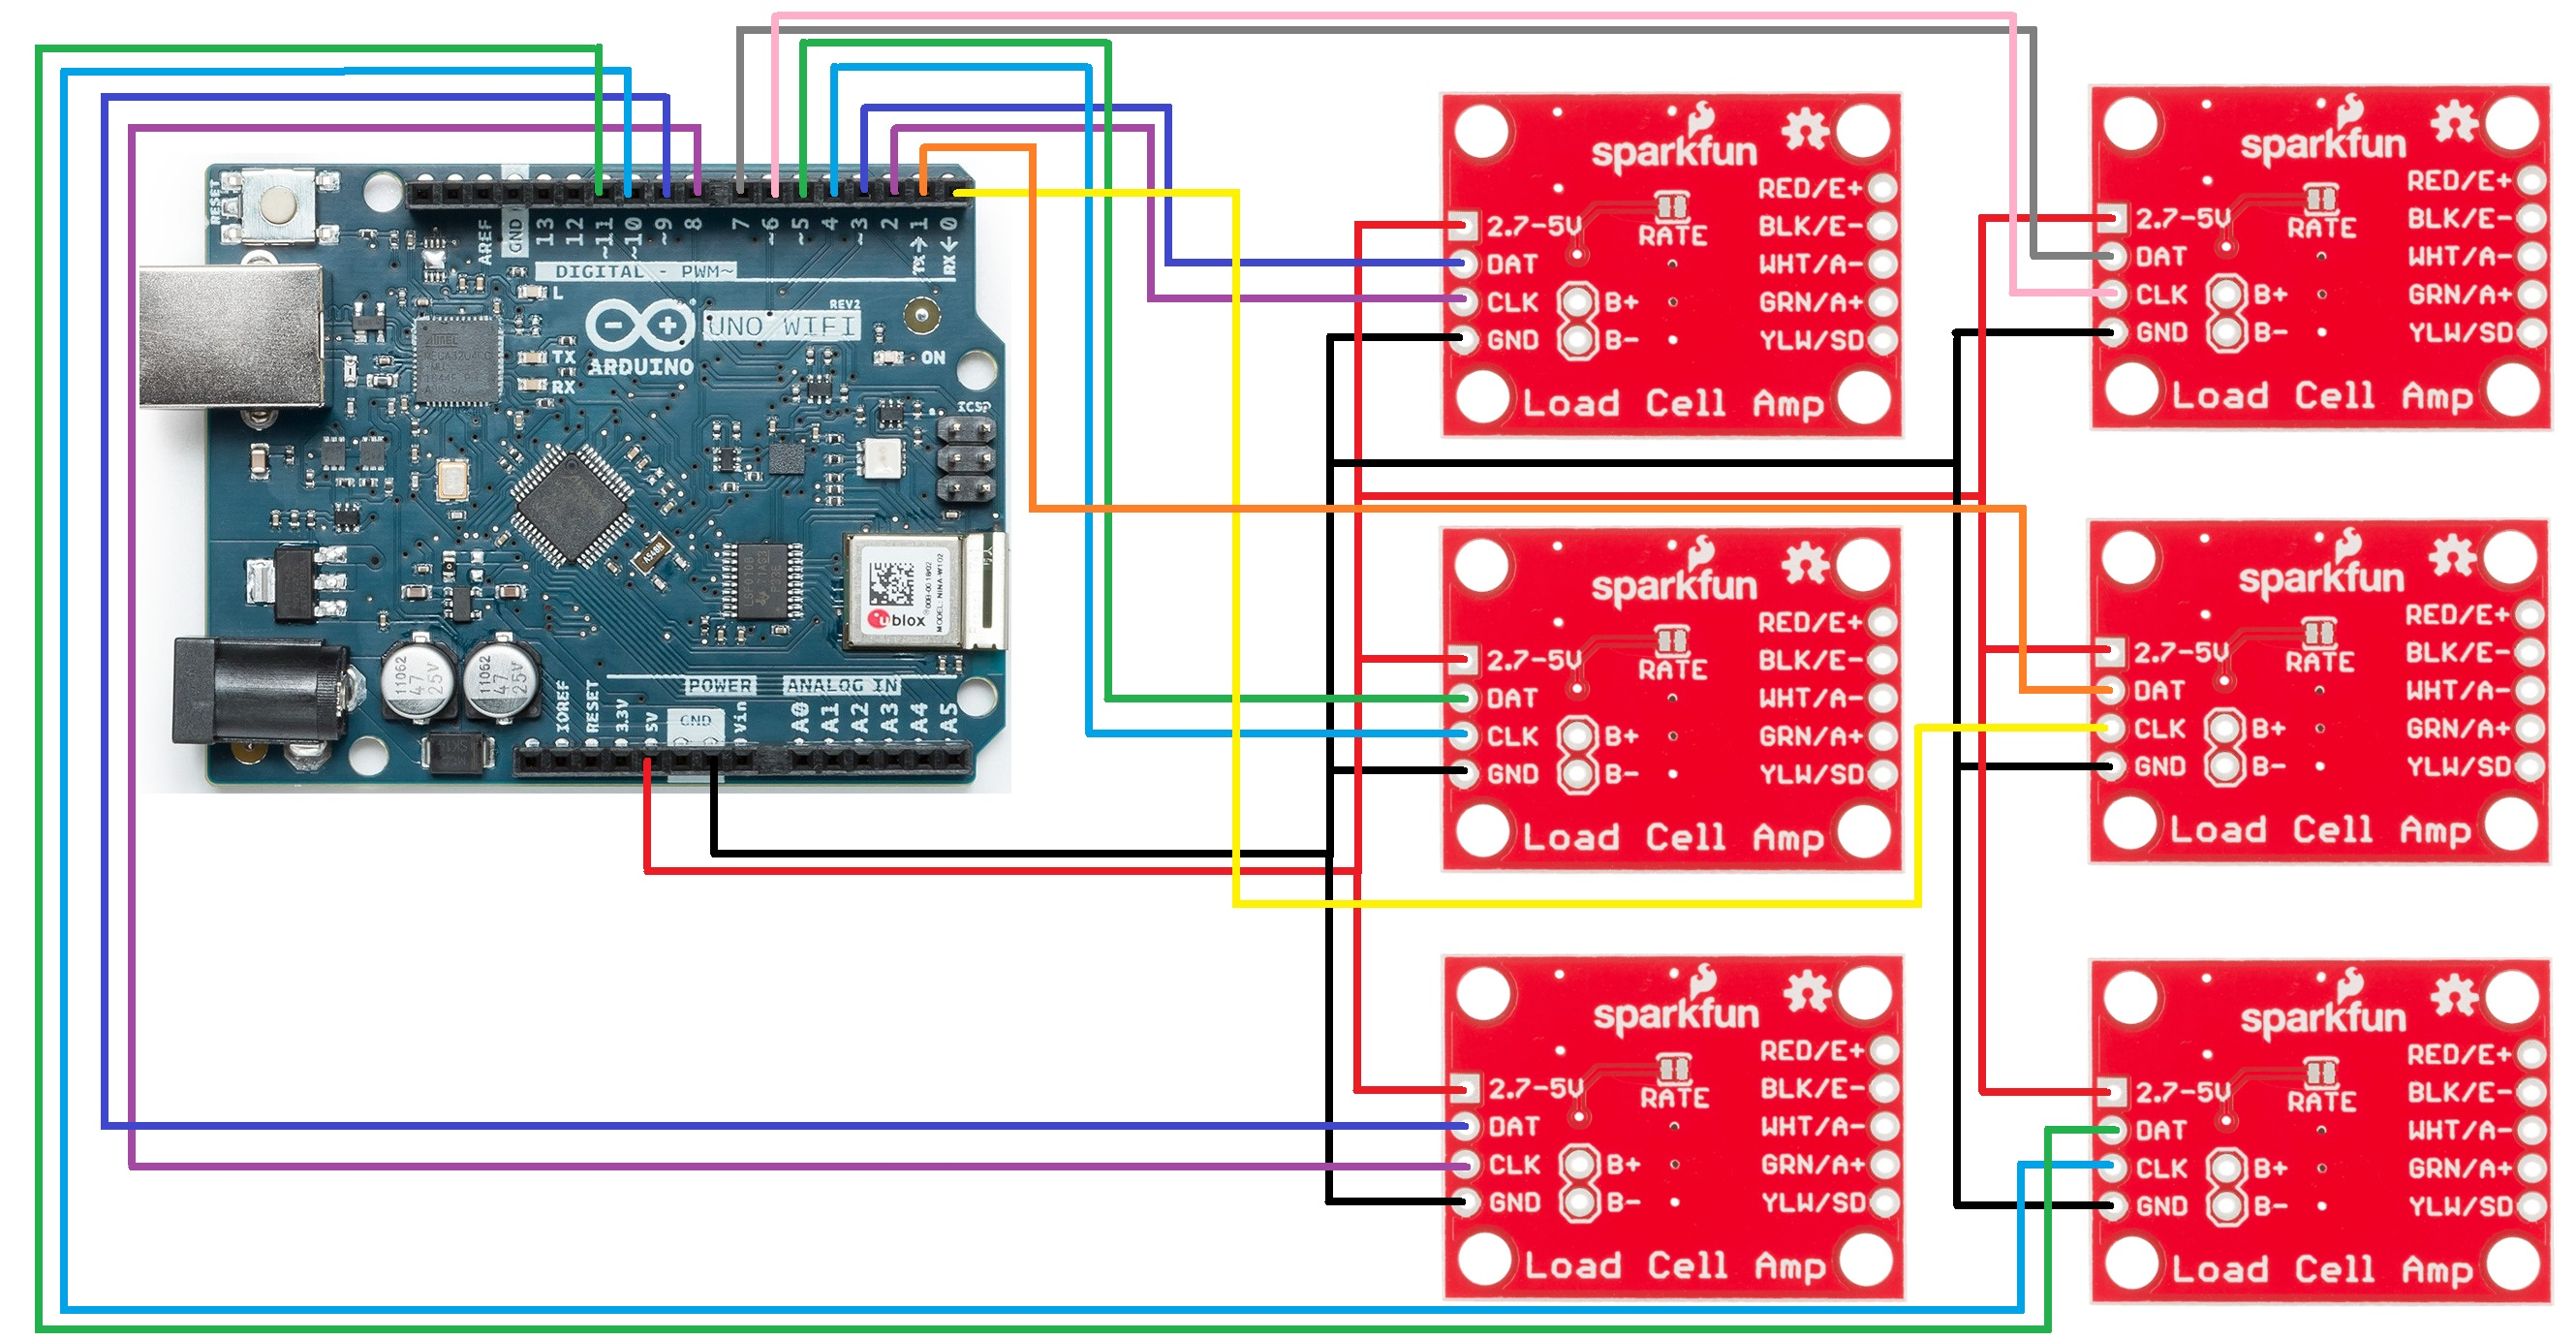
\includegraphics[width=.60\textwidth]{capitulos/capitulo6/ard4.jpg}
    \caption{Conexión entre Arduino y sensores de los basares.}
    \label{fig:ard4}
\end{figure}

Como se puede ver, cada peso está conectado a una toma a tierra (GND) y a una toma de 5V para la alimentación, luego el pin de los datos de cada peso es el pin digital 1, 3, 5, 7, 9 y 11 respectivamente, siendo el pin digital 0, 2, 4, 6, 8 y 10 para el reloj.

\subsection{Quinto controlador}

El quinto controlador se va a encargar de gestionar el contenido de los dos cajones de la fruta, es decir, va a gestionar los datos de dos pesos. Éste tendrá la IP \textbf{192.168.1.230} y se comunicará con el back-end a través del puerto \textbf{41328}. La conexión de los pines que hay entre estos dos sensores y el quinto controlador es la que se puede apreciar en la Figura \ref{fig:ard5}.

\begin{figure}[h] 
    \centering
    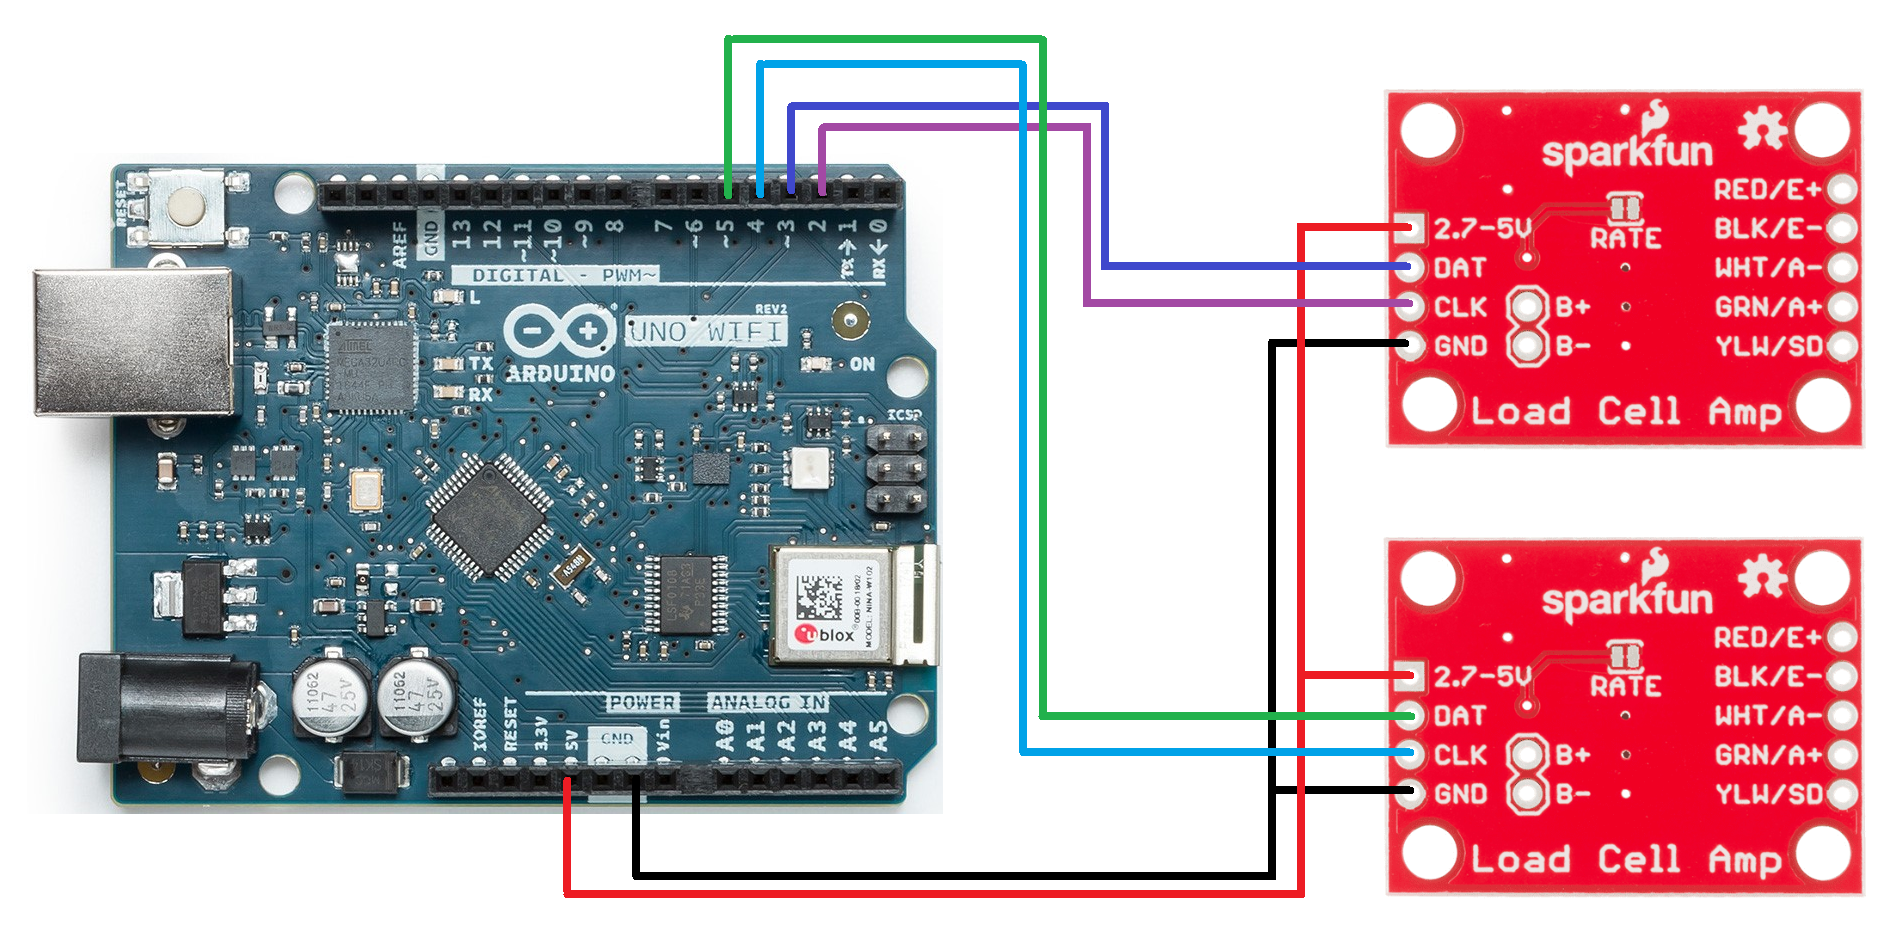
\includegraphics[width=.60\textwidth]{capitulos/capitulo6/ard2.png}
    \caption{Conexión entre Arduino y sensores del cajón de fruta.}
    \label{fig:ard5}
\end{figure}

Como se puede ver, cada peso está conectado a una toma a tierra (GND) y a una toma de 5V para la alimentación, luego un peso tiene su pin del reloj al pin digital 2, y el de datos al pin digital 3, el otro peso, el reloj al pin digital 4, y el de datos al pin digital 5.

\section{Código de los controladores}

Cada controlador tendrá su código propio que dependerá de los sensores que tenga conectados, aunque es cierto que todos los controladores tienen un principio de código que se repite, y es la parte donde se incluyen las librerías necesarias, se crean las variables necesarias, y se conecta a la red con la IP y el puerto especificado para comunicarse con el back-end. 

También hay un pequeño código en común que envía un paquete al back-end para avisar de que el controlador sigue con energía. Si ese paquete no llega cada cierto tiempo, el back-end entiende que ese controlador no tiene energía y enviará un aviso al usuario.

Después de esto, dependiendo de los sensores que tenga conectados, se va a hacer una cosa u otra, por lo que a continuación se va a explicar que pasos se seguirían dependiendo del sensor que esté conectado en el controlador. En caso de que un controlador tenga más de un sensor del mismo tipo conectado, va a hacer las mismas acciones, pero multiplicadas por el número de sensores iguales que tenga conectado.

\subsection{Sensor de peso}
Si se tiene un sensor de peso conectado, se va a estar leyendo el estado del sensor constantemente, y éste se va a comparar con la lectura anterior. Si existe una diferencia de 30g entre la medida actual y la anterior, se va a enviar la lectura nueva del sensor, si no es diferente, va a seguir cogiendo lecturas del sensor y comparando. La diferencia que tendrá que existir entre la medida actual y la anterior será adaptado al objeto que se está pesando cuando éste no es adecuado usar 30g, por ejemplo, si se coge solo una loncha de embutido.

\begin{figure}[h]
    \centering
    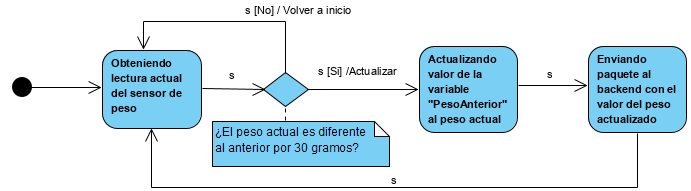
\includegraphics[width=.80\textwidth]{capitulos/capitulo6/diagramaPeso.png}
    \caption{Diagrama del proceso a seguir en un controlador con el sensor de peso.}
    \label{fig:diagramapeso}
\end{figure}

\subsection{Sensor de nivel}
Si el sensor conectado es un sensor de nivel de agua conectado, se va a estar leyendo el estado del sensor constantemente, y éste se va a comparar con la lectura anterior. Si es diferente, se va a enviar la lectura nueva del sensor, si no es diferente, va a seguir cogiendo lecturas del sensor y comparando. 

\begin{figure}[h]
    \centering
    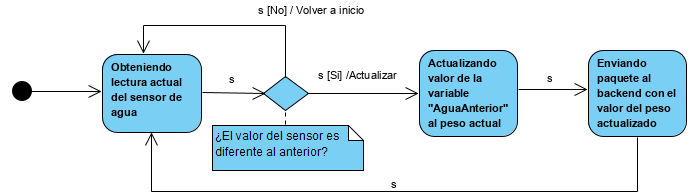
\includegraphics[width=.80\textwidth]{capitulos/capitulo6/diagramaNivelAgua.png}
    \caption{Diagrama del proceso a seguir en un controlador con el sensor de nivel de agua.}
    \label{fig:diagramaagua}
\end{figure}

\newpage
\subsection{Receptor del sensor magnético}
Si el sensor conectado es sensor magnético conectado, se va a estar leyendo el estado del sensor constantemente, y éste se va a comparar con la lectura anterior. Si es diferente, se va a enviar la lectura nueva del sensor, si no es diferente, va a seguir cogiendo lecturas del sensor y comparando. 

\begin{figure}[h]
    \centering
    \includegraphics[width=.80\textwidth]{capitulos/capitulo6/diagramaSensorMagnético.png}
    \caption{Diagrama del proceso a seguir en un controlador con el sensor magnético.}
    \label{fig:diagramamagnetico}
\end{figure}


\subsection{Sensor RFID}
Si se tiene un sensor RFID conectado, cuando una tarjeta pase por el lector se va a detectar si tiene contenido. 

\begin{itemize}
    \item Si tiene contenido, dependerá del que tenga:
    \begin{itemize}
        \item \textbf{Si es un producto}, se va a entender que el producto está siendo sacado del frigorífico y se va a eliminar el contenido de la tarjeta y enviar la confirmación de la eliminación del producto de la tarjeta al back-end.
        \item \textbf{Si es un usuario}, se puede querer eliminar el contenido de la tarjeta, o usar el contenido para loguear al usuario de dentro, por lo que primero se va a enviar una petición al back-end para saber si se quiere eliminar el contenido. 
        \begin{itemize}
            \item Si la respuesta es sí, se elimina el contenido y se envía la confirmación al back-end de eliminado.
            \item Si la respuesta es no, se lee la tarjeta para loguear al usuario que esta en el interior y se envía al back-end.
        \end{itemize}
    \end{itemize}
    \item Si no tiene contenido, se entiende que se quiere registrar algo en ella, así que se va a enviar una petición al back-end para que envíe el contenido a añadir a la tarjeta (que será un producto o un usuario). Cuando llegue, se escribe el contenido en la tarjeta y se envía la confirmación al back-end de que se ha escrito correctamente en la tarjeta.
\end{itemize}

\begin{landscape}
    \vspace*{7em}
\begin{figure}[h]
    \centering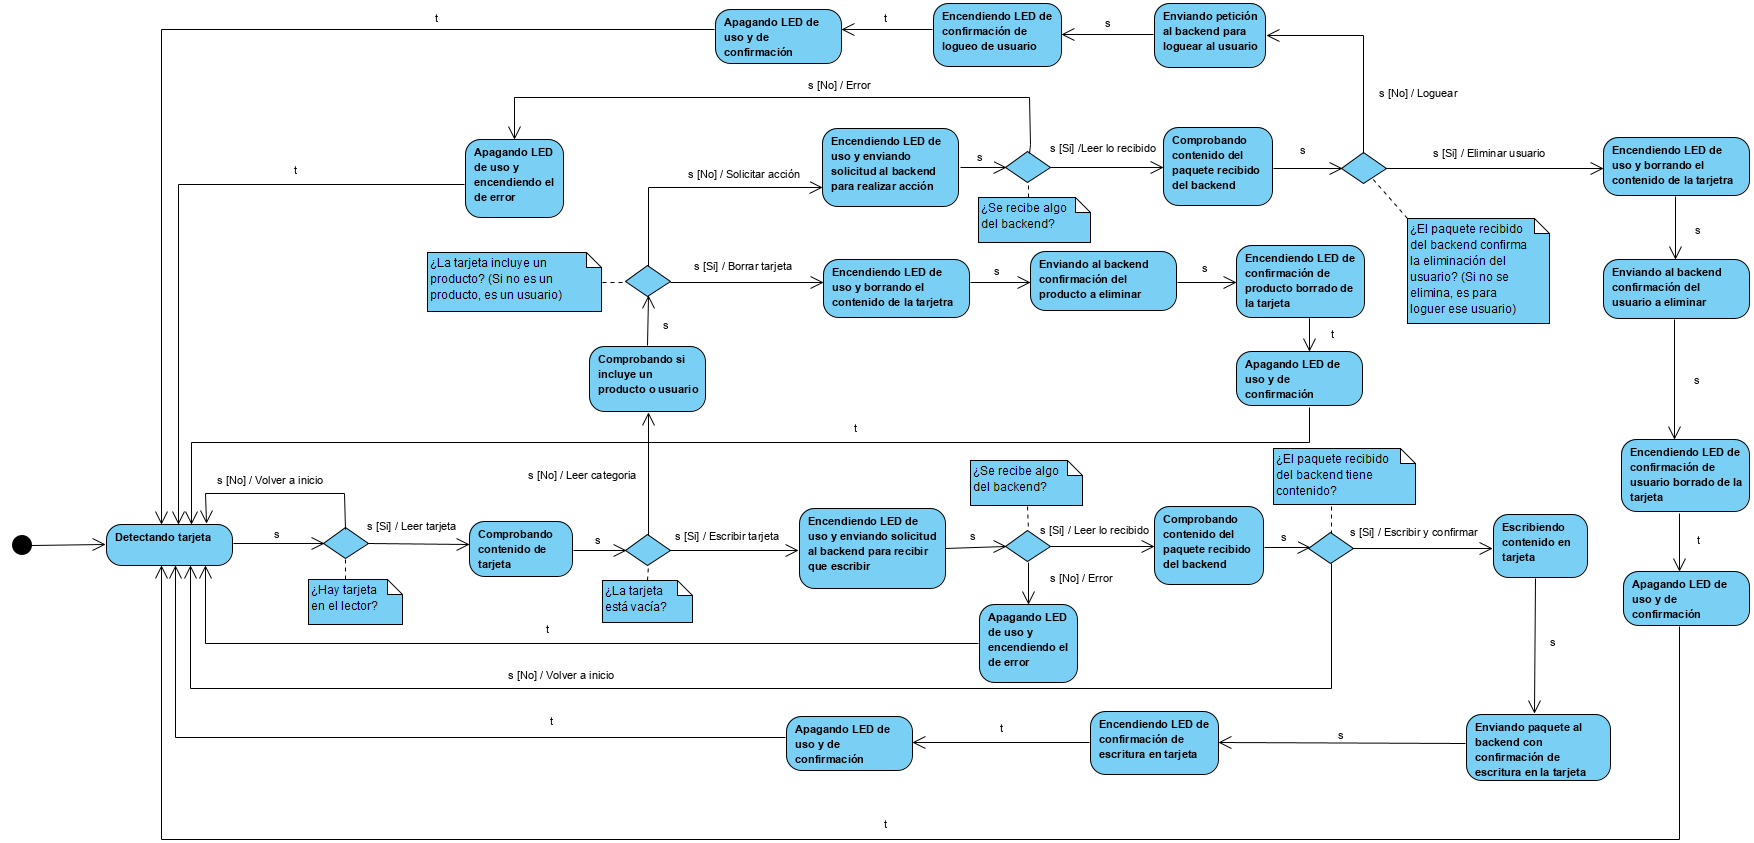
\includegraphics[width=\hsize]{capitulos/capitulo6/diagramaRFID.png}
    \caption{Diagrama del proceso a seguir en un controlador con el sensor RFID.}
    \label{img_gantt}
\end{figure}

\end{landscape}

\section{Localización}

Sabiendo la posición en la que van los sensores y cuales de ellos van conectados a que controlador, se puede identificar la localización de cada uno de éstos:

\begin{itemize}
    \item \textbf{Primer controlador:} Para el sensor RFID que va a estar en el exterior del frigorífico, se va a utilizar el primer controlador, y estará situado al lado del frigorífico.
    \item \textbf{Segundo controlador:} Este controlador va a ser usado por los sensores del cajón de verdura, situado detrás de los cajones para darle servicio.
    \item \textbf{Tercer controlador:} Para los sensores del cajón de embutido, para el sensor del nivel del agua y para los receptores de los sensores magnéticos habrá otra Arduino en el interior del cajón de embutidos.
    \item \textbf{Cuarto controlador:} Para lo sensores de peso de los basares, usarán el cuarto controlador guardado en el primer basar del frigorífico.
    \item \textbf{Quinto controlador:} Los sensores del cajón de fruta tendrán el quinto controlador, situado detrás de los cajones para darle servicio.
\end{itemize}

Se puede apreciar la localización de los controladores en el frigorífico en la Figura \ref{fig:controllerlg}. También todos los controladores que están dentro del frigorífico serán alimentadas con un soporte de 2 baterías 18650, un soporte con el de la Figura \ref{fig:battery}.

\begin{figure}[h] 
    \centering
    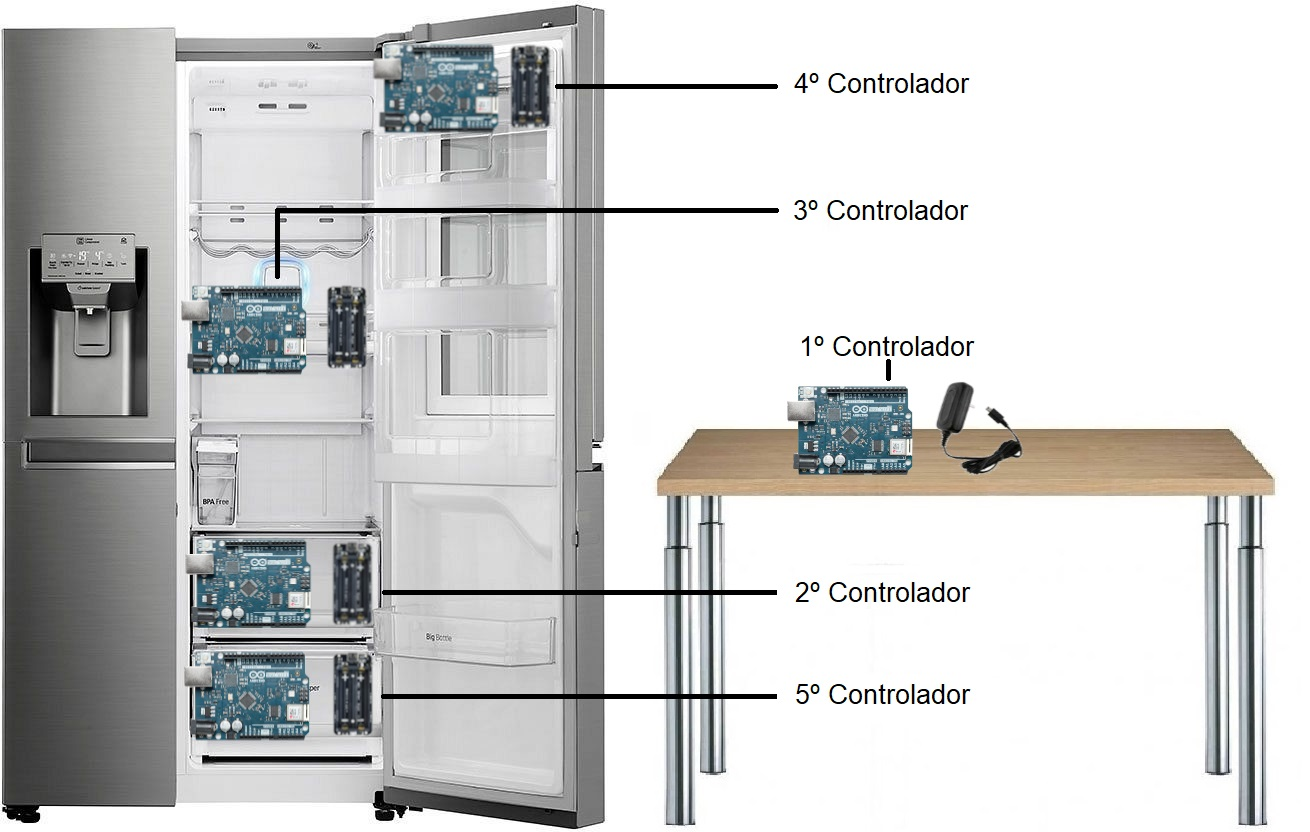
\includegraphics[width=.80\textwidth]{capitulos/capitulo6/controladorlg.jpg}
    \caption{Controladores instalados en el frigorífico.}
    \label{fig:controllerlg}
\end{figure}

\begin{figure}[h] 
    \centering
    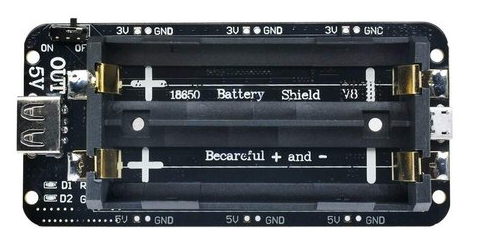
\includegraphics[width=.40\textwidth]{capitulos/capitulo6/battery.png}
    \caption{Soporte de baterías para Arduino.}
    \label{fig:battery}
\end{figure}

\newpage
\section{Presupuesto}
El presupuesto necesario para poder obtener los controladores y sus fuentes de energía se puede ver en la Tabla \ref{tab:resupuestocontrolador}.

\begin{table}[h]
    \centering
    \begin{tabular}{|l|c|c|c|}
        \rowcolor[gray]{.5}
        \hline
            \color{white}Artículo&\color{white}Precio&\color{white}Cantidad&\color{white}Subtotal  \\
        \hline
            Arduino Uno&25 euros &1&25 euros  \\
        \hline    
            Arduino Uno WiFi rev2&50 euros &5&250 euros  \\
        \hline    
            Soporte de batería&12 euros &4&48 euros  \\
         \hline   
            Batería 18650&3 euros &8&24 euros  \\
        \rowcolor[gray]{.9}
         \hline
            Total&-&18&347 euros  \\
        \hline
    \end{tabular}
    \caption{Presupuesto de la capa de neblina o niebla}
    \label{tab:resupuestocontrolador}
\end{table}

Como se muestra en la tabla, teniendo en cuenta todos los controladores y baterías necesarias para la realización de este proyecto, es necesario \textbf{347 euros} para poder conseguir desarrollar esta capa.